\section{A ficticious perfect cache}
In our first analysis we look at our four investigations from a first seen / last seen event perspective. We define a model where a ficticious perfect infinate cache is usesed. Every time a piece of data is first seen, its data size is added to the cache. Every time its last seen its removed out of the chache. The folowing diagrams show the probability density function of the required amount of RAM to implement such a perfect disk cache in. 
\begin{figure}
\centering
\subfloat[case 1]{
  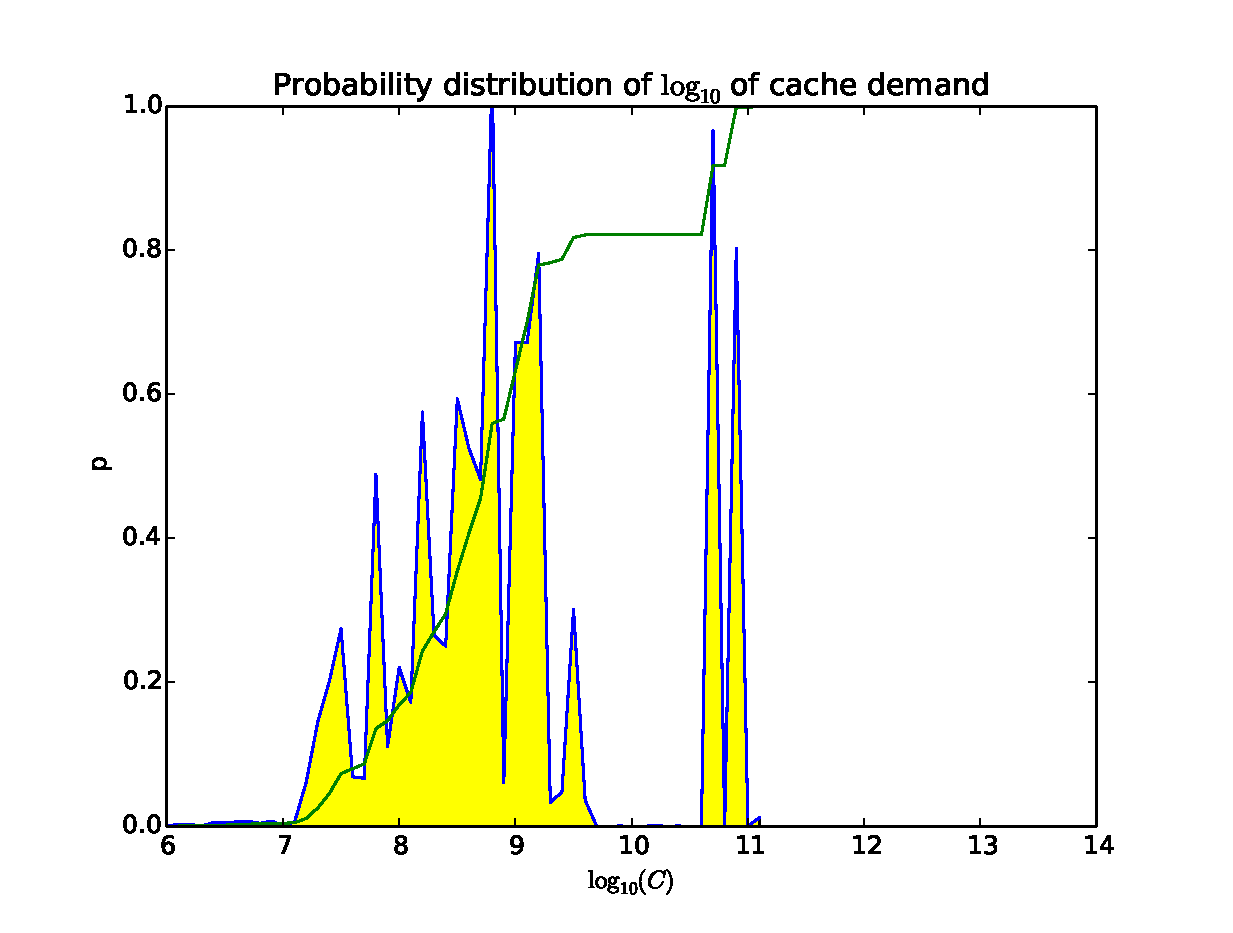
\includegraphics[width=70mm]{ocfa/step2/stripped1_virtcachesize.eps}
}
\subfloat[case 2]{
  \includegraphics[width=70mm]{ocfa/step2/stripped2_virtcachesize.eps}
}
\hspace{0mm}
\subfloat[case 3]{
  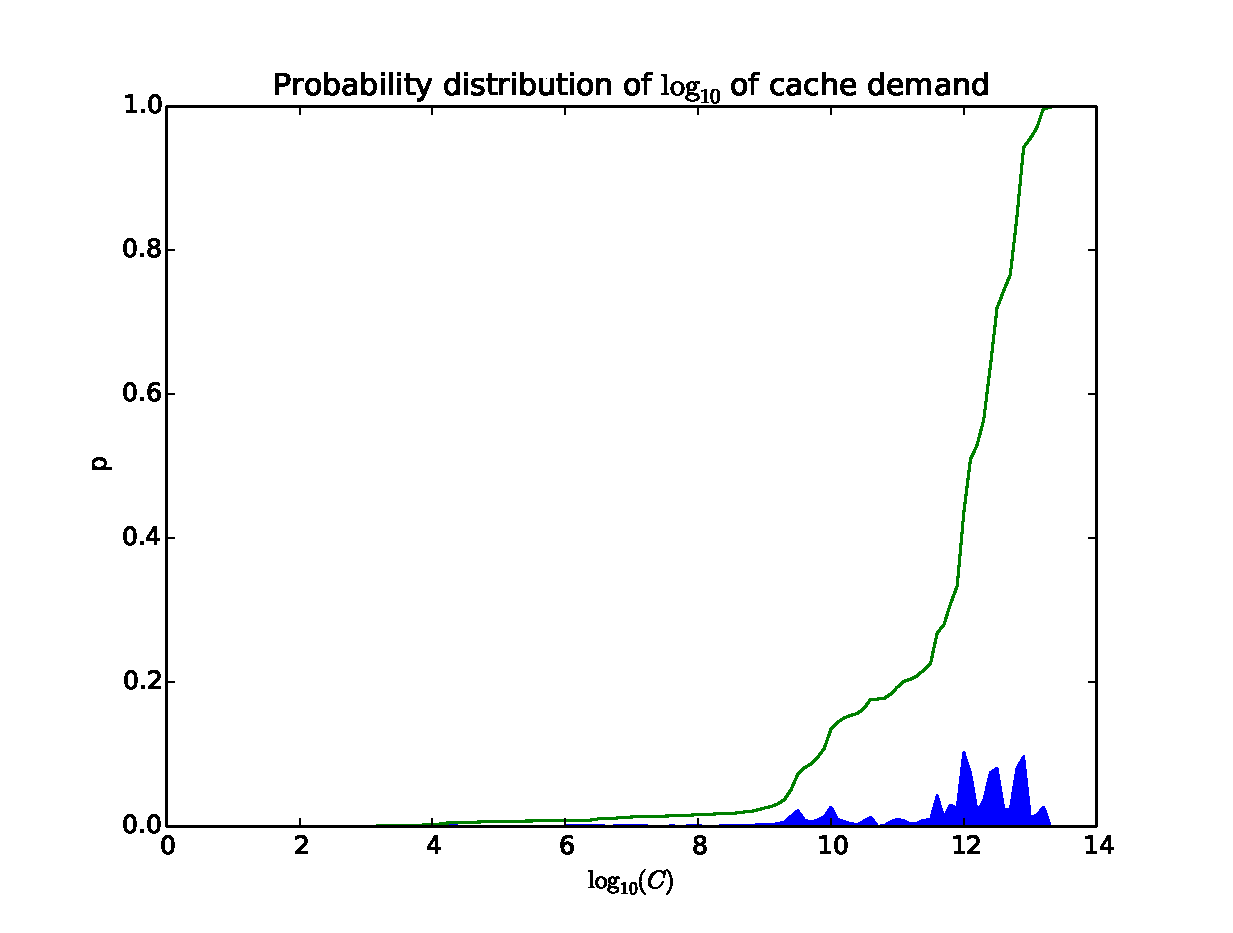
\includegraphics[width=70mm]{ocfa/step2/stripped3_virtcachesize.eps}
}
\subfloat[case 4]{
  \includegraphics[width=70mm]{ocfa/step2/stripped4_virtcachesize.eps}
}
\caption{Virtual cache size propability density}
\end{figure}
